\documentclass[letterpaper,11pt]{article}
\oddsidemargin -1.0cm \textwidth 17.5cm

\usepackage[utf8]{inputenc}
\usepackage[activeacute,spanish, es-lcroman]{babel}
\decimalpoint
\usepackage{amsfonts,setspace}
\usepackage{amsmath}
\usepackage{amssymb, amsmath, amsthm}
\usepackage{comment}
\usepackage{float}
\usepackage{amssymb}
\usepackage{dsfont}
\usepackage{anysize}
\usepackage{multicol}
\usepackage{enumerate}
\usepackage{graphicx}
\usepackage[left=1.5cm,top=2cm,right=1.5cm, bottom=1.7cm]{geometry}
\setlength\headheight{1.5em} 
\usepackage{fancyhdr}
\usepackage{multicol}
\usepackage{hyperref}
\usepackage{wrapfig}
\usepackage{subcaption}
\usepackage{siunitx}
\usepackage{cancel}
\pagestyle{fancy}
\fancyhf{}
\renewcommand{\labelenumi}{\normalsize\bfseries P\arabic{enumi}.}
\renewcommand{\labelenumii}{\normalsize\bfseries (\alph{enumii})}
\renewcommand{\labelenumiii}{\normalsize\bfseries \roman{enumiii})}


\begin{document}

\fancyhead[L]{\itshape{Facultad de Ciencias F\'isicas y Matem\'aticas}}
\fancyhead[R]{\itshape{Universidad de Chile}}

\begin{minipage}{11.5cm}
    \begin{flushleft}
        \hspace*{-0.6cm}\textbf{FI1000-6 Introducción a la Física Clásica}\\
        \hspace*{-0.6cm}\textbf{Profesora:} Paulina Lira\\
        \hspace*{-0.6cm}\textbf{Auxiliares:} Juan Cristóbal Castro \& Alejandro Silva\\
        \hspace*{-0.6cm}\textbf{Ayudantes:} Catalina Molina \& Francisca Bórquez\\
        
    \end{flushleft}
\end{minipage}

\begin{picture}(2,3)
    \put(366, 10){
\includegraphics[scale=0.9]{2020-1/Imágenes/logo/dfi-fcfm.pdf}}
\end{picture}

\begin{center}
	\LARGE\textbf{Auxiliar \#0}\\
	\Large{Trigonometría}
\end{center}

\vspace{-1cm}
\begin{enumerate}\setlength{\itemsep}{0.4cm}

\rfoot[]{pág. \thepage}

\item[]

\item Dos observadores $A$ y $B$ miden ángulos de elevación de un avión que los sobrevuela a una altura constante. En cierto instante los ángulos medidos por $A$ y $B$ son $\alpha = 60^{\circ}$ y $\beta = 40^{\circ}$, respectivamente. La separación entre $A$ y  $B$ es $D = \SI{1}{\km}$. ¿A qué altura vuela el avión?

\begin{figure}[h!]
    \centering
    \begin{subfigure}[t]{0.4\textwidth}
        \centering
        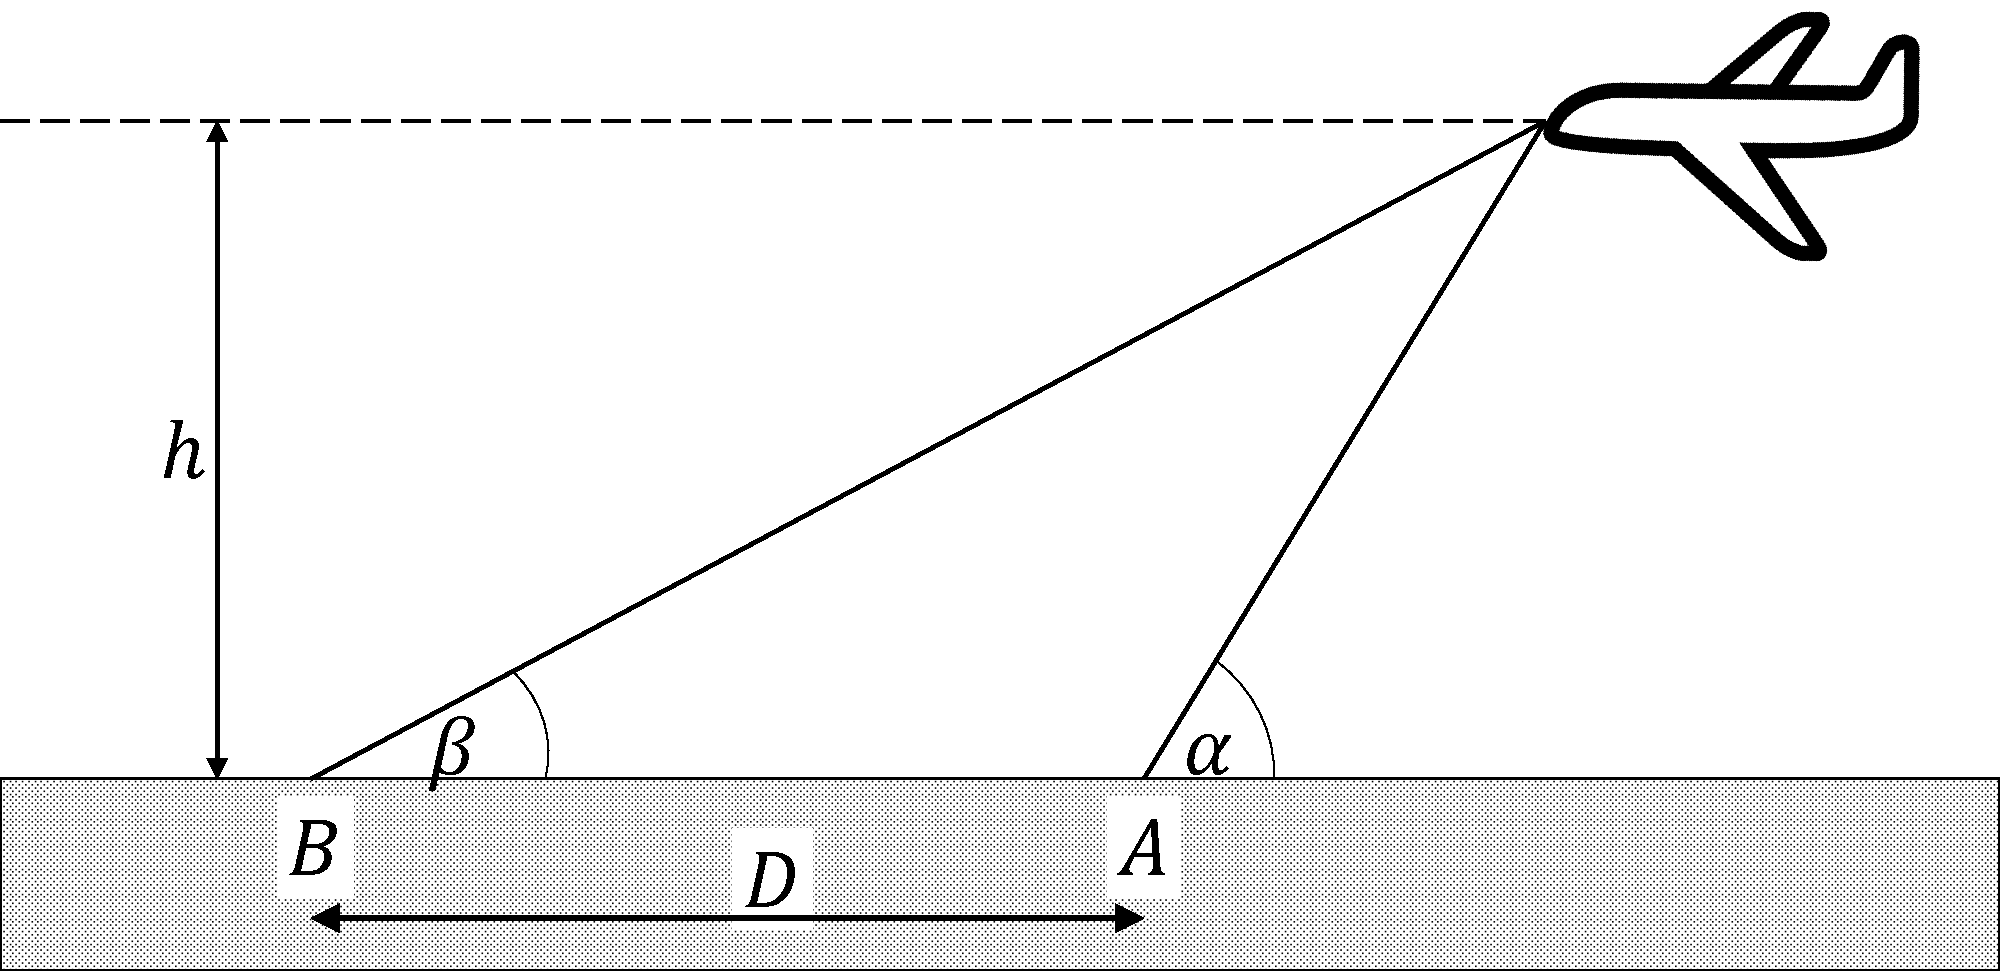
\includegraphics[width=0.8\linewidth]{2021-1/Imagenes/aux0/avion.pdf}
        \caption*{Figura P1}
    \end{subfigure}
    \hspace{0.5cm}
    \begin{subfigure}[t]{0.4\textwidth}
        \centering
        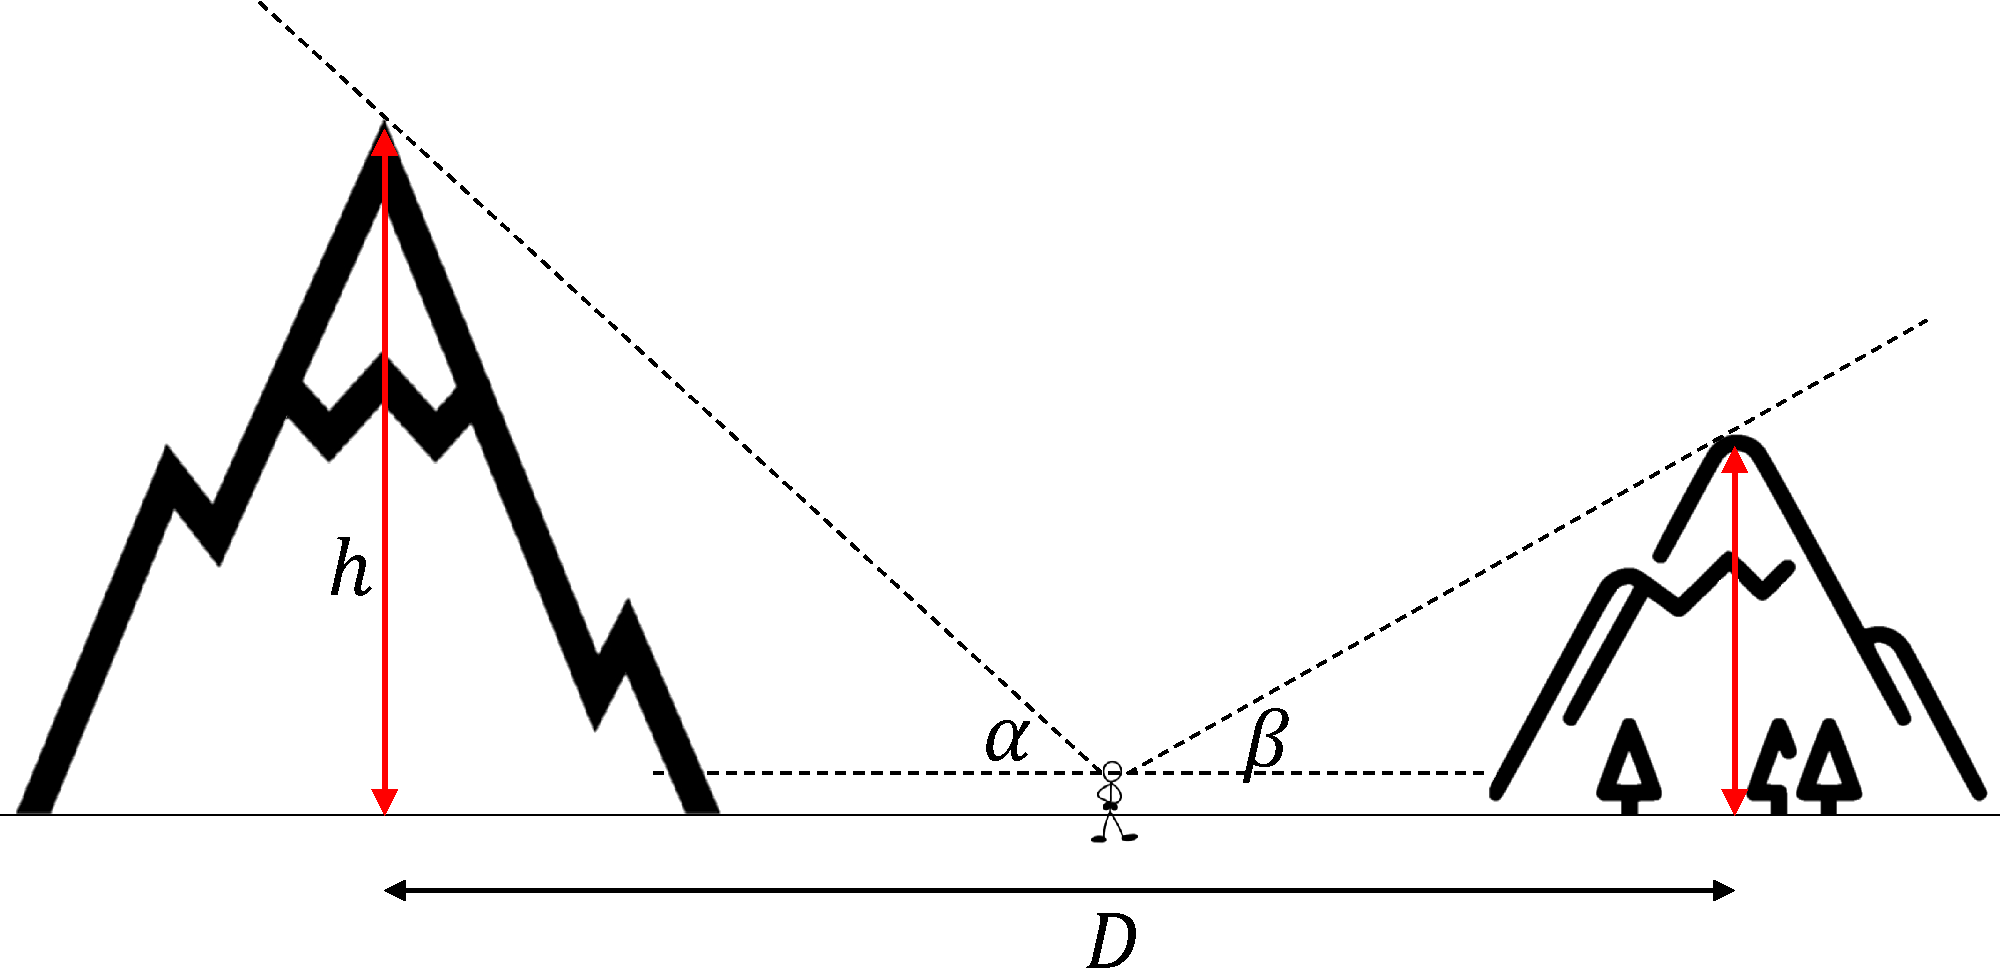
\includegraphics[width=0.9\linewidth]{2021-1/Imagenes/aux0/mountain.pdf}
        \caption*{Figura P2}
    \end{subfigure}
\end{figure}

\item Una persona ubicada en el punto $P$ observa dos montañas, una a la izquierda y otra a la derecha. Sean $\alpha$ y $\beta$ los ángulos de elevación de estas montañas. Si la montaña de la izquierda tiene una altura $h$ y la separación entre las proyecciones de las cimas sobre el nivel de la superficie terrestre es $D$, calcule la altura del otro monte. 

\item Demuestre el teorema del seno y del coseno para un triángulo acutángulo.\\
\textit{Hint:} forme triángulos rectángulos

\begin{figure}[H]
    \centering
    \begin{subfigure}[t]{0.4\textwidth}
        \centering
        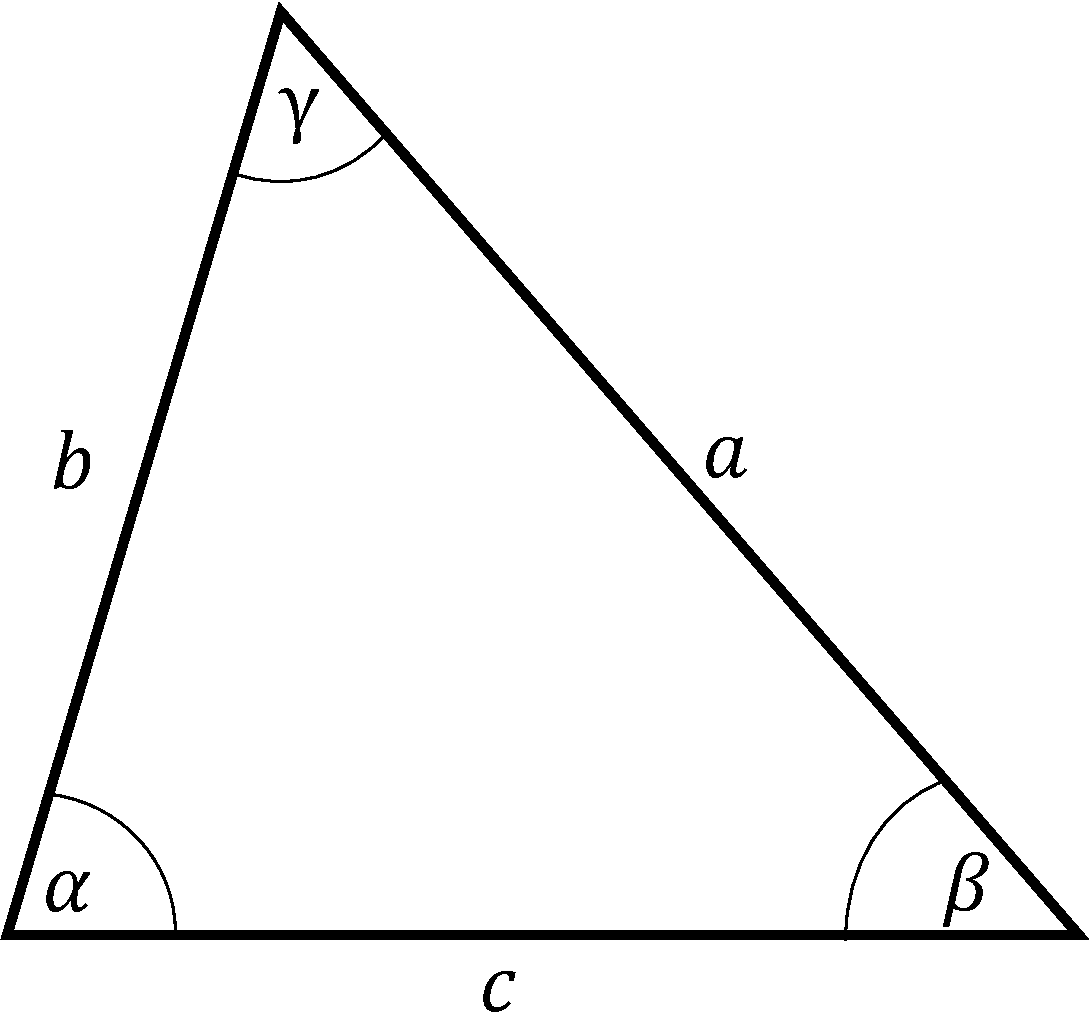
\includegraphics[width=0.6\linewidth]{2021-1/Imagenes/aux0/acutangulo.pdf}
    \end{subfigure}
    \hspace{0.5cm}
    \begin{subfigure}[t]{0.4\textwidth}
        \vspace{-4cm}
        Teo. Seno:
        \begin{align*}
            \frac{\sin{\alpha}}{a} = \frac{\sin{\beta}}{b} = \frac{\sin{\gamma}}{c}
        \end{align*}
        
        Teo.Coseno
        \begin{align*}
            a^2 = b^2 + c^2 - 2bc \cos{\alpha}\\
            b^2 = a^2 + c^2 - 2ac \cos{\beta}\\
            c^2 = a^2 + b^2 - 2ab \cos{\gamma}
        \end{align*}
    \end{subfigure}
    \caption*{Figura P3}
\end{figure}

\item Demuestre las siguientes relaciones trigonométricas:
    {
    \begin{multicols}{2}
        \begin{enumerate}
        \item $\sin^2\alpha = \cfrac{1 - \cos{(2\alpha)}}{2}$
        
        \item $\tan^2\alpha + 1 = sec^2\alpha$
        
        \columnbreak
        
        \item $\sin\alpha + \sin\beta = 2\sin{\left(\cfrac{\alpha+\beta}{2}\right)}\cos{\left(\cfrac{\alpha-\beta}{2}\right)}$
        
        \item $\cos\alpha+\cos\beta = 2\cos{\left(\cfrac{\alpha+\beta}{2}\right)}\cos{\left(\cfrac{\alpha-\beta}{2}\right)}$
    \end{enumerate}
    \end{multicols}
    }


\end{enumerate}
\end{document}